\section{Within-Universe Factor-Mimicking Portfolios}
\label{app:within-univ}

Because the 30-stock universe is concentrated in mega-cap technology, global Fama--French factors may not capture style tilts that occur \emph{within} the universe.
For each characteristic $c$, we construct a monthly within-universe long--short portfolio by sorting the 30 stocks on $c$, going long the top 6 (on the traditional ``long'' side of that characteristic) and short the bottom 6, rebalancing with a 2-day lag and no transaction cost.
Table~\ref{tab:within-univ-corr} reports the daily-return Pearson correlation between each LLM's Q1$-$Q5 portfolio and these factor-mimicking portfolios (expected-return mode).

\begin{table}[H]
\centering
\caption{Correlation between LLM Q1$-$Q5 returns and within-universe factor-mimicking portfolios. Positive entries align with the factor's traditional long side; stars test zero correlation with Newey--West HAC SE: $^{*}p<0.10$, $^{**}p<0.05$, $^{***}p<0.01$.}
\label{tab:within-univ-corr}
\scriptsize
\setlength{\tabcolsep}{3pt}
\resizebox{\textwidth}{!}{
\begin{tabular}{l lllllll}
\toprule
\textbf{Model} & Mom & Rev & LowVol & E/P & ROE & LowInv & SmallSize \\
\midrule
GPT-4o & \multicolumn{1}{l}{$-$0.02} & \multicolumn{1}{l}{$-$0.04} & \multicolumn{1}{l}{$-$0.18$^{**}$} & \multicolumn{1}{l}{$-$0.18$^{**}$} & \multicolumn{1}{l}{$-$0.10} & \multicolumn{1}{l}{$-$0.13$^{*}$} & \multicolumn{1}{l}{$-$0.23$^{***}$} \\
GPT-4o mini & \multicolumn{1}{l}{$-$0.20$^{***}$} & \multicolumn{1}{l}{$+$0.22$^{***}$} & \multicolumn{1}{l}{$+$0.22$^{***}$} & \multicolumn{1}{l}{$+$0.21$^{***}$} & \multicolumn{1}{l}{$-$0.00} & \multicolumn{1}{l}{$+$0.20$^{***}$} & \multicolumn{1}{l}{$+$0.11$^{*}$} \\
GPT-4.1 & \multicolumn{1}{l}{$+$0.37$^{***}$} & \multicolumn{1}{l}{$-$0.38$^{***}$} & \multicolumn{1}{l}{$-$0.70$^{***}$} & \multicolumn{1}{l}{$-$0.57$^{***}$} & \multicolumn{1}{l}{$-$0.31$^{***}$} & \multicolumn{1}{l}{$-$0.47$^{***}$} & \multicolumn{1}{l}{$-$0.29$^{***}$} \\
GPT-4.1 mini & \multicolumn{1}{l}{$+$0.29$^{***}$} & \multicolumn{1}{l}{$-$0.39$^{***}$} & \multicolumn{1}{l}{$-$0.12} & \multicolumn{1}{l}{$-$0.16} & \multicolumn{1}{l}{$-$0.02} & \multicolumn{1}{l}{$-$0.02} & \multicolumn{1}{l}{$-$0.20$^{***}$} \\
GPT-4.1 nano & \multicolumn{1}{l}{$+$0.13} & \multicolumn{1}{l}{$-$0.21$^{**}$} & \multicolumn{1}{l}{$-$0.23$^{**}$} & \multicolumn{1}{l}{$-$0.13} & \multicolumn{1}{l}{$-$0.08} & \multicolumn{1}{l}{$-$0.08} & \multicolumn{1}{l}{$-$0.18$^{**}$} \\
o4-mini & \multicolumn{1}{l}{$+$0.24$^{**}$} & \multicolumn{1}{l}{$-$0.11} & \multicolumn{1}{l}{$-$0.65$^{***}$} & \multicolumn{1}{l}{$-$0.46$^{***}$} & \multicolumn{1}{l}{$-$0.29$^{***}$} & \multicolumn{1}{l}{$-$0.28$^{***}$} & \multicolumn{1}{l}{$-$0.24$^{***}$} \\
o3 & \multicolumn{1}{l}{$+$0.28$^{***}$} & \multicolumn{1}{l}{$-$0.15} & \multicolumn{1}{l}{$-$0.80$^{***}$} & \multicolumn{1}{l}{$-$0.60$^{***}$} & \multicolumn{1}{l}{$-$0.35$^{***}$} & \multicolumn{1}{l}{$-$0.49$^{***}$} & \multicolumn{1}{l}{$-$0.29$^{***}$} \\
\midrule
Gem. 2.5 Flash & \multicolumn{1}{l}{$+$0.48$^{***}$} & \multicolumn{1}{l}{$-$0.32$^{***}$} & \multicolumn{1}{l}{$-$0.54$^{***}$} & \multicolumn{1}{l}{$-$0.57$^{***}$} & \multicolumn{1}{l}{$-$0.21$^{***}$} & \multicolumn{1}{l}{$-$0.23$^{**}$} & \multicolumn{1}{l}{$-$0.17$^{**}$} \\
Gem. 2.5 Pro & \multicolumn{1}{l}{$+$0.44$^{***}$} & \multicolumn{1}{l}{$-$0.13} & \multicolumn{1}{l}{$-$0.78$^{***}$} & \multicolumn{1}{l}{$-$0.67$^{***}$} & \multicolumn{1}{l}{$-$0.42$^{***}$} & \multicolumn{1}{l}{$-$0.34$^{***}$} & \multicolumn{1}{l}{$-$0.14$^{**}$} \\
\midrule
Cl. Sonnet 4 & \multicolumn{1}{l}{$+$0.37$^{***}$} & \multicolumn{1}{l}{$-$0.34$^{***}$} & \multicolumn{1}{l}{$-$0.50$^{***}$} & \multicolumn{1}{l}{$-$0.53$^{***}$} & \multicolumn{1}{l}{$-$0.21$^{***}$} & \multicolumn{1}{l}{$-$0.40$^{***}$} & \multicolumn{1}{l}{$-$0.27$^{***}$} \\
Cl. Opus 4 & \multicolumn{1}{l}{$+$0.51$^{***}$} & \multicolumn{1}{l}{$-$0.23$^{**}$} & \multicolumn{1}{l}{$-$0.59$^{***}$} & \multicolumn{1}{l}{$-$0.61$^{***}$} & \multicolumn{1}{l}{$-$0.24$^{***}$} & \multicolumn{1}{l}{$-$0.42$^{***}$} & \multicolumn{1}{l}{$-$0.20$^{***}$} \\
\bottomrule
\end{tabular}
}
\end{table}

The correlation structure is consistent with the FF6 loadings in Table~\ref{tab:ff6} and the style fingerprint in Figure~\ref{fig:style}: the strongest representative models---o3, Gemini 2.5 Pro, and Claude Opus 4---all show positive momentum correlation and negative low-volatility/value correlations, confirming a high-momentum, high-volatility growth tilt within the universe.
GPT-4o mini remains the main counterexample, with negative momentum and positive reversal/low-volatility correlations, consistent with its anti-monotonic quintile pattern during the 2024--2025 AI rally.

Figure~\ref{fig:loadings} visualizes the FF6 factor loadings as a heatmap, offering a compact view of the cross-vendor style differences.

\begin{figure}[H]
  \centering
  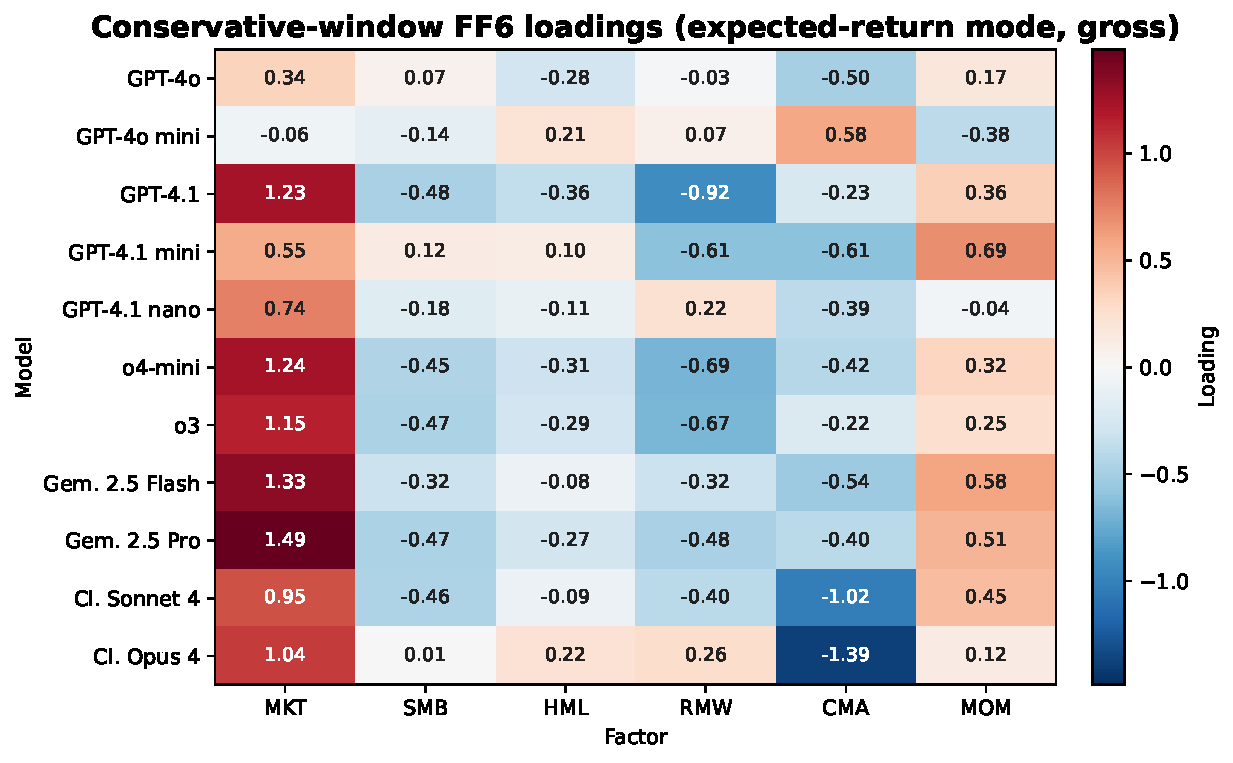
\includegraphics[width=\columnwidth]{figures/fig9_factor_loadings.pdf}
  \caption{Conservative-window FF6 factor loadings of expected-return Q1$-$Q5 portfolios. Red indicates positive loading and blue indicates negative loading.}
  \Description{Heatmap of Fama-French six-factor loadings for current expected-return long-short portfolios, with red for positive loadings and blue for negative loadings.}
  \label{fig:loadings}
\end{figure}

The heatmap closes the appendix by linking the table-level style correlations back to the FF6 spanning tests.
Across the stronger expected-return rankers, positive market and momentum exposure coexists with negative value/profitability/investment loadings, consistent with the growth--momentum implicit-prior interpretation developed in the main text.